\section{ALGORITMA DAN LOGIKA APLIKASI}

Bab ini menjelaskan logika inti Savora: \textit{Food Trust Index} (penilaian kelayakan berbasis
input UMKM), \textit{Food Score Decay} (skor kelayakan yang meluruh terhadap waktu), \textit{Keyword
Classification} (klasifikasi keamanan dari ulasan), \textit{Dynamic Discount} (rekomendasi diskon),
serta perhitungan \textit{service fee} pada pembayaran \textit{cashless}. Seluruh logika dirancang
\textit{rule-based} (deterministik) sehingga transparan, \textit{explainable}, dapat diaudit, dan
dapat dihitung \textit{real-time} tanpa layanan \textit{machine learning} terpisah.

\subsection{Prioritas Implementasi Fitur}

Tabel~\ref{tab:implementasi} merangkum status implementasi fitur utama, konsisten dengan ruang
lingkup MVP (lihat bab Ruang Lingkup dan Batasan Perangkat Lunak).

\begin{table}[htbp]
\centering
\caption{Status Implementasi Fitur}
\label{tab:implementasi}
\small
\begin{tabularx}{\textwidth}{|l|X|l|}
\hline
\textbf{Modul} & \textbf{Fitur} & \textbf{Status} \\
\hline
\multirow{6}{*}{UMKM} & Kelola produk (reguler \& mystery box) & Sudah berjalan \\
\cline{2-3}
& Food Score Decay & Sudah berjalan \\
\cline{2-3}
& Dashboard analitik \& insight & Sudah berjalan \\
\cline{2-3}
& Iklan produk & Sudah berjalan \\
\cline{2-3}
& Kelola status pesanan & Sudah berjalan \\
\cline{2-3}
& Food Trust Index (input UMKM) \& Waste Log & Direncanakan \\
\hline
\multirow{4}{*}{Customer} & Marketplace \& Food Score live & Sudah berjalan \\
\cline{2-3}
& Keyword classification ulasan & Sudah berjalan \\
\cline{2-3}
& Checkout cashless (Midtrans) + service fee 5\% & Direncanakan \\
\cline{2-3}
& Pesanan, pickup code, Help Center & Direncanakan \\
\hline
\multirow{2}{*}{Auth} & Login / Register (4 role) & Direncanakan \\
\cline{2-3}
& Role-based access & Direncanakan \\
\hline
Admin & Verifikasi UMKM/Mitra Donasi, keuangan, moderasi & Direncanakan \\
\hline
\multirow{2}{*}{Lanjutan} & Dynamic pricing otomatis (ML) & Roadmap \\
\cline{2-3}
& Prediksi permintaan (ML), real-time & Roadmap \\
\hline
\end{tabularx}
\end{table}

\subsection{Food Trust Index}

Food Trust Index (FTI) adalah penilaian kelayakan makanan berbasis aturan yang dihitung dari input
UMKM saat membuat listing. FTI bersifat transparan dan \textit{explainable}, bukan sertifikasi
laboratorium, dan tidak menggantikan pemeriksaan langsung customer saat pickup.

\subsubsection{Input dan Output}

Input FTI meliputi kategori makanan, waktu masak/produksi, metode penyimpanan, kondisi kemasan, dan
ada/tidaknya kuah/saus. Berdasarkan akumulasi indikasi risiko dari input tersebut, sistem
memetakan produk ke salah satu dari lima status pada Tabel~\ref{tab:fti}.

\begin{table}[htbp]
\centering
\caption{Output Food Trust Index}
\label{tab:fti}
\small
\begin{tabularx}{\textwidth}{|l|X|l|}
\hline
\textbf{Status} & \textbf{Makna (berdasarkan input UMKM)} & \textbf{Aksi Sistem} \\
\hline
Fresh & Makanan baru, kemasan baik, penyimpanan sesuai & Publikasikan \\
\hline
Layak Dijual & Masih dalam estimasi masa simpan, tanpa indikasi risiko & Publikasikan \\
\hline
Segera Dijual & Mendekati batas waktu konsumsi, kemasan masih memadai & Publikasikan + urgency \& diskon tinggi \\
\hline
Tidak Disarankan Dijual & Indikasi risiko sedang (penyimpanan/waktu kurang ideal) & Tidak tampil; evaluasi internal \\
\hline
Tidak Layak Konsumsi & Indikasi risiko tinggi (lewat masa/kemasan buruk) & Tidak tampil; arahkan ke Waste Log \\
\hline
\end{tabularx}
\end{table}

\subsubsection{Aturan Penilaian}

Penilaian menggunakan pendekatan sederhana yang dapat dijelaskan ke juri: setiap indikator input
diberi bobot risiko; akumulasi risiko rendah menghasilkan status \emph{Fresh}/\emph{Layak Dijual},
risiko sedang menghasilkan \emph{Segera Dijual}/\emph{Tidak Disarankan Dijual}, dan risiko tinggi
menghasilkan \emph{Tidak Layak Konsumsi}. Setiap detail produk wajib menampilkan \textit{disclaimer}
bahwa FTI dihitung dari informasi UMKM dan aturan platform, dan customer tetap disarankan memeriksa
kondisi makanan saat pickup. Status FTI juga berperan sebagai skor awal/plafon ($S_0$) bagi
perhitungan Food Score Decay pada subbab berikut.

\subsection{Food Score Decay}

Food Score adalah indikator kelayakan makanan bernilai 0--100 yang menurun seiring
berkurangnya sisa waktu rescue menuju batas kedaluwarsa. Model ini mengacu pada konsep
\textit{freshness index} / masa simpan makanan \textit{perishable}: kesegaran cenderung bertahan
di awal masa simpan lalu turun lebih cepat menjelang batas layak konsumsi, sehingga kurvanya
sedikit konveks \cite{iotshelflife2025}.

\subsubsection{Rumus}

Misalkan $t_{r}$ adalah sisa waktu rescue, $W$ adalah lebar jendela rescue (nilai $t_{r}$ saat
produk pertama dimuat), dan $S_{0}$ adalah skor awal/plafon dari UMKM (mis. Food Trust Index,
maksimum 100). Fraksi kesegaran didefinisikan sebagai:

\begin{equation}
f = \frac{\max(0,\ \min(t_{r},\ W))}{W}, \qquad 0 \le f \le 1
\end{equation}

Food Score dihitung dengan peluruhan berpangkat (\textit{power decay}):

\begin{equation}
\mathrm{FES} = \operatorname{round}\!\left( S_{0} \cdot f^{\,\gamma} \right), \qquad \gamma = 0.65
\end{equation}

Eksponen $\gamma = 0.65$ ($<1$) membuat kurva konveks: skor bertahan relatif tinggi di awal dan
turun lebih tajam menjelang kedaluwarsa. Sebagai contoh, pada $S_{0}=100$: saat $f=0{,}5$ maka
$\mathrm{FES}\approx 64$, dan saat $f=0{,}2$ maka $\mathrm{FES}\approx 35$. Gambar~\ref{fig:decay}
menampilkan profil peluruhan tersebut.

\begin{figure}[htbp]
\centering
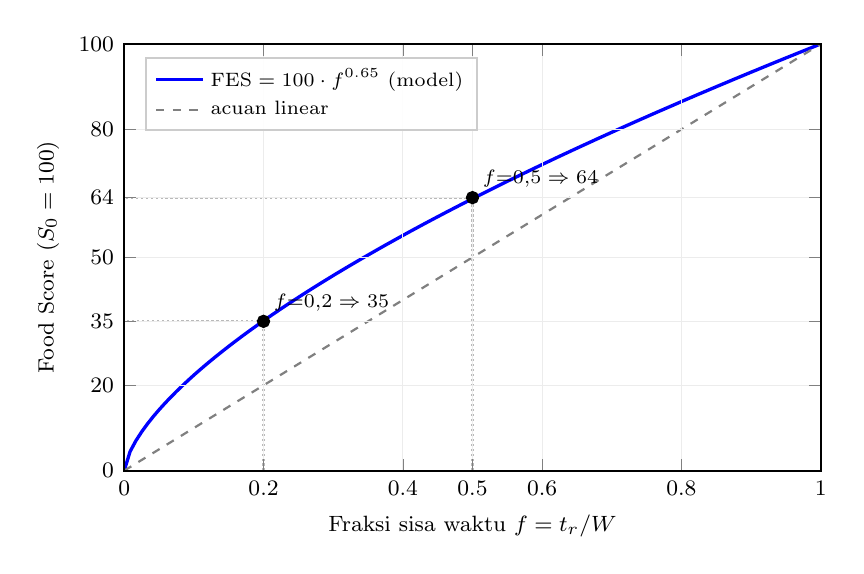
\begin{tikzpicture}
\begin{axis}[
    width=0.86\textwidth, height=7cm,
    xlabel={Fraksi sisa waktu $f = t_r / W$},
    ylabel={Food Score ($S_0=100$)},
    xmin=0, xmax=1, ymin=0, ymax=100,
    xtick={0,0.2,0.4,0.5,0.6,0.8,1},
    ytick={0,20,35,50,64,80,100},
    grid=both, grid style={gray!15}, minor tick num=0,
    domain=0:1, samples=120,
    thick, font=\footnotesize,
    legend pos=north west,
    legend cell align=left,
    legend style={draw=gray!40, font=\scriptsize, fill=white, fill opacity=0.9, text opacity=1},
    axis on top,
]
% Power-decay curve (the model)
\addplot[blue, very thick] {100*(x^0.65)};
\addlegendentry{$\mathrm{FES}=100\cdot f^{0.65}$ (model)}
% Linear reference for contrast
\addplot[gray, dashed, thick] {100*x};
\addlegendentry{acuan linear}
% Example points cited in the text, with guide lines and labels
\addplot[only marks, mark=*, mark size=2pt, black] coordinates {(0.5,64) (0.2,35)};
\draw[gray!55, densely dotted] (axis cs:0.5,0) -- (axis cs:0.5,64) -- (axis cs:0,64);
\draw[gray!55, densely dotted] (axis cs:0.2,0) -- (axis cs:0.2,35) -- (axis cs:0,35);
\node[anchor=south west, font=\scriptsize] at (axis cs:0.5,64) {$f{=}0{,}5\Rightarrow 64$};
\node[anchor=south west, font=\scriptsize] at (axis cs:0.2,35) {$f{=}0{,}2\Rightarrow 35$};
\end{axis}
\end{tikzpicture}
\caption{Kurva Peluruhan Food Score ($\gamma=0.65$): skor bertahan tinggi di awal lalu turun lebih tajam mendekati kedaluwarsa}
\label{fig:decay}
\end{figure}

\subsubsection{Band Skor}

Skor dipetakan ke band kelayakan yang tampil ke pengguna beserta warna statusnya, sesuai ambang
pada kode:

\begin{table}[htbp]
\centering
\caption{Band Food Score}
\label{tab:fes_band}
\small
\begin{tabularx}{\textwidth}{|l|l|X|}
\hline
\textbf{Rentang Skor} & \textbf{Label} & \textbf{Makna} \\
\hline
$\ge 80$ & Sangat Layak & Kualitas masih prima \\
\hline
$60$--$79$ & Layak & Aman dikonsumsi \\
\hline
$35$--$59$ & Segera Ambil & Disarankan segera diambil \\
\hline
$1$--$34$ & Kritis & Mendekati batas kelayakan \\
\hline
$0$ & Kedaluwarsa & Melewati batas rescue \\
\hline
\end{tabularx}
\end{table}

\subsubsection{Alur Perhitungan}

\begin{figure}[htbp]
\centering
\begin{tikzpicture}[
    font=\scriptsize, node distance=0.75cm,
    io/.style={draw, trapezium, trapezium left angle=70, trapezium right angle=110, fill=blue!8, align=center, minimum height=0.8cm, text width=3.4cm, inner sep=2pt},
    proc/.style={draw, rounded corners, fill=green!8, align=center, minimum height=0.8cm, text width=3.2cm},
    dec/.style={draw, diamond, aspect=2, fill=orange!12, align=center, inner sep=1pt},
    flow/.style={-{Latex}, thick},
]
\node[io] (in) {Input: $t_r$, $W$, $S_0$};
\node[proc, below=of in] (frac) {Hitung fraksi $f=\dfrac{t_r}{W}$ (clamp $0..1$)};
\node[proc, below=of frac] (calc) {$\mathrm{FES}=\operatorname{round}(S_0\cdot f^{0.65})$};
\node[proc, below=of calc] (band) {Petakan ke band skor};
\node[io, below=of band] (out) {Output: skor + label};

\draw[flow] (in) -- (frac);
\draw[flow] (frac) -- (calc);
\draw[flow] (calc) -- (band);
\draw[flow] (band) -- (out);
\end{tikzpicture}
\caption{Flowchart Perhitungan Food Score}
\label{fig:fes_flow}
\end{figure}

\subsection{Keyword Classification dari Ulasan}

Selain rating numerik, Savora mengklasifikasikan keyword pada ulasan customer untuk membangun
sinyal keamanan makanan per UMKM secara \textit{crowdsourced}. Mesin klasifikasi bersifat
\textit{rule-based} dan telah tersedia pada basis kode (\textit{frontend}).

\subsubsection{Kamus dan Tingkat Keamanan}

Keyword dipetakan ke tiga tingkat keamanan dengan peringkat (\textit{rank}) berbeda, sebagaimana
Tabel~\ref{tab:keyword}. Jika sebuah ulasan memuat beberapa keyword sekaligus, tingkat paling gawat
yang menang (prinsip \textit{worst-case}).

\begin{table}[htbp]
\centering
\caption{Tingkat Keamanan Keyword Ulasan}
\label{tab:keyword}
\small
\begin{tabularx}{\textwidth}{|l|l|X|}
\hline
\textbf{Level} & \textbf{Rank} & \textbf{Contoh Keyword} \\
\hline
Gawat & 3 & basi, berjamur, busuk, beracun, keracunan, kadaluarsa \\
\hline
Warning & 2 & bau, asam, tengik, apek, lembek, kurang segar \\
\hline
Aman & 1 & enak, segar, fresh, lezat, bersih, higienis, gurih \\
\hline
\end{tabularx}
\end{table}

\subsubsection{Agregasi ke Badge UMKM}

Untuk setiap UMKM, sistem menghitung jumlah ulasan per level dan mengambil level terburuk yang
muncul sebagai badge keamanan (Aman/Warning/Gawat). Bila tersedia level yang telah dihitung
\textit{backend} (mis. via \texttt{keyword\_scores}), nilai tersebut diprioritaskan; jika tidak,
sistem melakukan agregasi lokal dari daftar ulasan. Badge ini ditampilkan pada kartu dan halaman
detail UMKM sehingga customer memperoleh sinyal keamanan tambahan sebelum bertransaksi.

\subsection{Dynamic Discount dan Perhitungan Harga}

Pada MVP, harga rescue ($p_{r}$) ditetapkan oleh UMKM saat membuat produk. Sistem memberikan
\emph{rekomendasi} rentang diskon berdasarkan status Food Trust Index (mis. \emph{Segera Dijual}
disarankan diskon 35--50\%), namun keputusan akhir tetap di tangan UMKM dengan \textit{guardrail}
harga minimum agar tetap menguntungkan (\textit{time-aware manual pricing}). Sistem kemudian
menghitung besaran diskon dan penghematan secara otomatis dari harga asli ($p_{o}$) dan harga
rescue tersebut.

\subsubsection{Rumus}

\begin{equation}
\mathrm{diskon}\ (\%) = \operatorname{round}\!\left( \frac{p_{o} - p_{r}}{p_{o}} \times 100 \right), \qquad p_o > 0
\end{equation}

\begin{equation}
\mathrm{penghematan} = p_{o} - p_{r}
\end{equation}

Nilai diskon di-\textit{clamp} agar tidak negatif. Diskon dan penghematan inilah yang ditampilkan
pada kartu produk di marketplace, berdampingan dengan Food Score dan \textit{countdown}
sisa waktu rescue.

\subsubsection{Alur Penetapan Harga}

\begin{figure}[htbp]
\centering
\begin{tikzpicture}[
    font=\scriptsize, node distance=0.7cm,
    io/.style={draw, trapezium, trapezium left angle=70, trapezium right angle=110, fill=blue!8, align=center, minimum height=0.8cm, text width=4cm, inner sep=2pt},
    proc/.style={draw, rounded corners, fill=green!8, align=center, minimum height=0.8cm, text width=3.6cm},
    flow/.style={-{Latex}, thick},
]
\node[io] (in) {UMKM tetapkan $p_r$ (mempertimbangkan sisa waktu \& margin)};
\node[proc, below=of in] (disc) {Hitung diskon\\$\operatorname{round}((p_o-p_r)/p_o\times100)$};
\node[proc, below=of disc] (save) {Hitung penghematan $p_o-p_r$};
\node[proc, below=of save] (show) {Tampilkan di marketplace bersama Food Score \& timer};
\node[io, below=of show] (out) {Customer melihat harga rescue};
\draw[flow] (in) -- (disc);
\draw[flow] (disc) -- (save);
\draw[flow] (save) -- (show);
\draw[flow] (show) -- (out);
\end{tikzpicture}
\caption{Flowchart Penetapan dan Perhitungan Harga Rescue}
\label{fig:pricing_flow}
\end{figure}

\subsubsection{Roadmap: Dynamic Pricing Otomatis}

Penetapan harga otomatis berbasis \textit{reinforcement learning} seperti \textit{Q-learning} untuk
meminimalkan food waste \cite{qlearning2026pricing} diposisikan sebagai pengembangan lanjutan
(\textit{out-of-scope} MVP). Pendekatan ini akan mengoptimalkan harga berdasarkan elastisitas
permintaan lokal dan sisa waktu kelayakan secara adaptif, menggantikan penetapan manual saat ini.

\subsection{Perhitungan Service Fee pada Pembayaran Cashless}

Model pendapatan utama Savora adalah \textit{service fee} 5\% per transaksi. Untuk sebuah pesanan
dengan subtotal produk $p_{r}$ (harga rescue $\times$ kuantitas), sistem menghitung:

\begin{equation}
\mathrm{service\_fee} = \operatorname{round}(0{,}05 \times \mathrm{subtotal}), \qquad
\mathrm{total} = \mathrm{subtotal} + \mathrm{service\_fee}
\end{equation}

Nilai \textit{service fee} dan total ditampilkan transparan di halaman checkout sebelum customer
membayar. Backend membuat token transaksi ke Midtrans \textit{sandbox} sebesar $\mathrm{total}$,
lalu memperbarui status pesanan menjadi \emph{Paid} hanya setelah menerima dan memverifikasi
notifikasi/\textit{signature} dari Midtrans. Setelah \emph{Paid}, sistem membuat \textit{pickup
code} unik untuk validasi pengambilan oleh UMKM, dan akumulasi \textit{service fee} dicatat pada
pendapatan platform (\texttt{platform\_revenue}).

\subsection{Integrasi Antar Komponen}
\begin{itemize}[leftmargin=*]
    \item \textbf{Frontend--Backend} : Komunikasi via RESTful API dengan format JSON.
    \item \textbf{Backend--Database} : Menggunakan GORM (ORM untuk Go) untuk akses PostgreSQL, termasuk \textit{auto-migration} skema.
    \item \textbf{Food Score} : Dihitung di sisi frontend secara \textit{rule-based} dan diperbarui \textit{real-time} mengikuti \textit{countdown} sisa waktu rescue.
    \item \textbf{Pembayaran} : Backend berkomunikasi dengan Midtrans \textit{sandbox} untuk membuat token transaksi dan memverifikasi notifikasi/\textit{webhook} sebelum memperbarui status order.
\end{itemize}
